\section{Diagrama Entidad-Relaci\'on}

% -----------------------------------------------------------------------------
\thispagestyle{empty}
  \begin{figure}[H] \centering
    \subfloat[der]
    {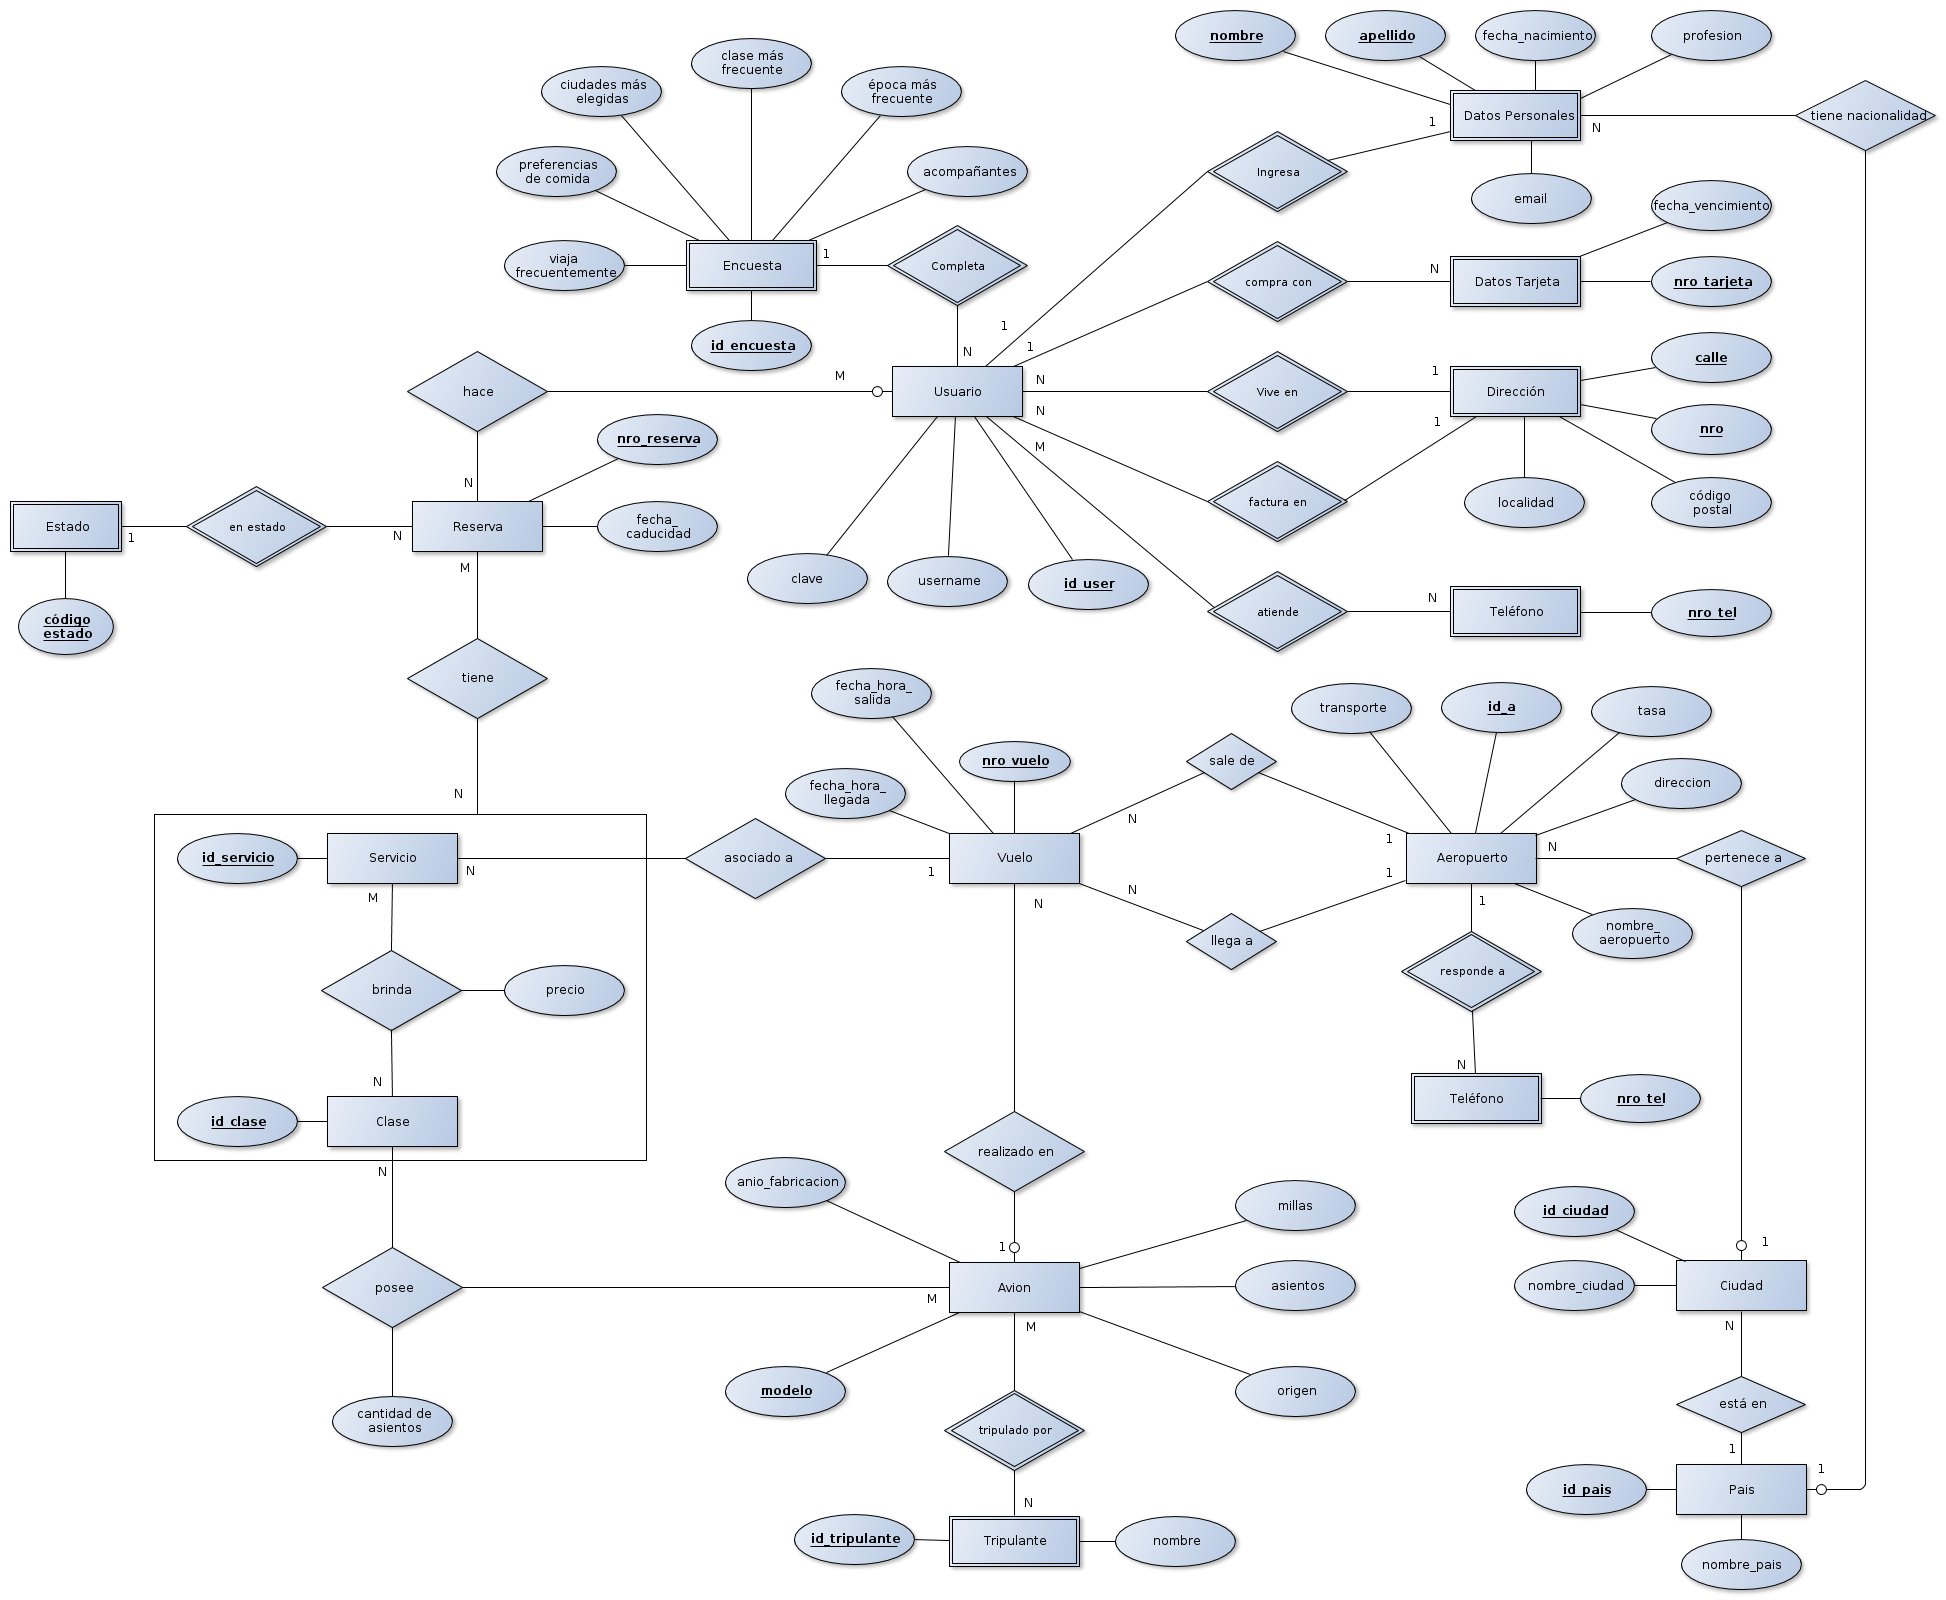
\includegraphics[width=\linewidth]{./img/der.png}}
    {}
  %\hspace*{6cm}
  \end{figure} 

% -----------------------------------------------------------------------------

\subsection{Aclaraciones}
  \begin{itemize}
    \item Consideramos que una reserva puede tener varios estados, estos son
          \begin{itemize}
            \item   Realizada
            \item   Cancelada
            \item   Confirmada
          \end{itemize}

          Las reservas realizadas pueden cancelarse o confirmarse.
          Es necesario confirmar una reserva para poder viajar.
          Para simplificar, suponemos que todos los usuarios con reservas
          confirmadas realizan efectivamente el viaje.
    
    \item La aerolínea ofrece servicios de viaje, y cada usuario realiza una
          reserva sobre un par de servicio-clase.
          De esta forma vemos la cantidad de asientos que está reservando por
          cada clase para un servicio.
          A la vez un servicio tiene varios vuelos (yo había entendido esto)

    \item Consideramos que los mensajes que el sistema la envía a los usuarios
          no son lo suficientemente relevantes para el problema que queremos
          modelar (????)
            
  \end{itemize}

\subsection{Restricciones}
  \begin{itemize}
    \item
    
    \item    
  \end{itemize}


